\documentclass[aspectratio=169,10pt]{beamer}

\usepackage[utf8]{inputenc}
\usepackage[T1]{fontenc}
\usepackage{lmodern}
\usepackage{microtype}
\usepackage{booktabs}
\usepackage{tabularx}
\usepackage{amsmath}
\usepackage{siunitx}
\usepackage{graphicx}
\usepackage{tikz}
\usepackage{xcolor}
\usepackage{hyperref}
\usetikzlibrary{positioning}

\usetheme{Madrid}
\setbeamertemplate{navigation symbols}{}
\setbeamertemplate{footline}[frame number]
\graphicspath{{../../thesis/figures/}}

\definecolor{PFBlue}{HTML}{28536B}
\definecolor{PFSand}{HTML}{C2944A}
\definecolor{PFGreen}{HTML}{567A3F}
\definecolor{PFGray}{HTML}{3A4351}
\definecolor{PFSoft}{HTML}{F5F1E8}

\setbeamercolor{title}{fg=PFBlue}
\setbeamercolor{frametitle}{fg=PFBlue}
\setbeamercolor{structure}{fg=PFBlue}
\setbeamercolor{block title}{fg=white,bg=PFBlue}
\setbeamercolor{block body}{fg=black,bg=PFSoft}

\title{PFUI fuer neue Gruppenmitglieder}
\subtitle{Lokale Analyse und Einzelinspektion von DFT-Datenbanken}
\author{Codex}
\institute{Onboarding fuer die Forschungsgruppe}
\date{\today}

\begin{document}

\begin{frame}
  \titlepage
\end{frame}

\begin{frame}{Ziel der Einfuehrung}
  \begin{block}{Nach der Praesentation sollen neue Studierende drei Dinge koennen}
    \begin{enumerate}
      \item lokale HDF-Datenbanken in PFUI laden und den Projektzustand verstehen
      \item einzelne DFT-Rechnungen fachlich sinnvoll inspizieren und kuratieren
      \item aus gefilterten Daten belastbare Tabellen und Plots fuer chemische Fragen ableiten
    \end{enumerate}
  \end{block}

  \vspace{0.4cm}
  \begin{itemize}
    \item Fokus: sichere Orientierung, nicht jedes Detail der Software
    \item Zielgruppe: Chemie-Studierende mit wenig Programmiererfahrung
    \item guter Einstieg: etwa 15 bis 20 Minuten Vortrag plus Live-Demo
  \end{itemize}
\end{frame}

\begin{frame}{Mentales Modell der Software}
  \centering
  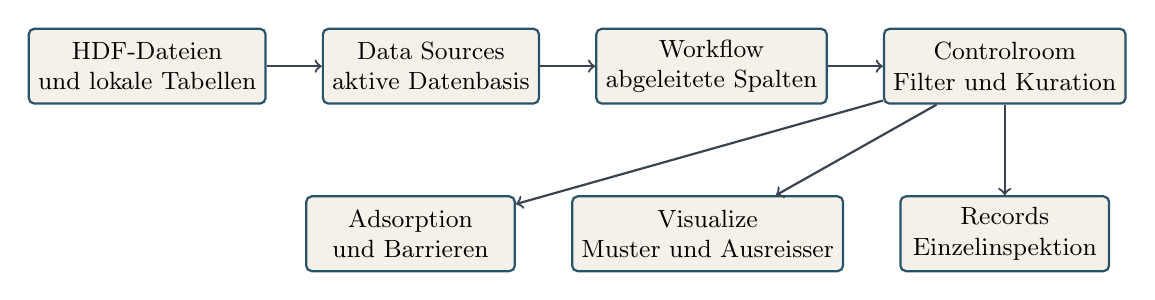
\begin{tikzpicture}[
    node distance=1.15cm and 0.7cm,
    every node/.style={font=\small, rounded corners=2pt, align=center},
    box/.style={draw=PFBlue, thick, fill=PFSoft, minimum width=2.65cm, minimum height=0.95cm},
    arrow/.style={->, thick, color=PFGray}
  ]
    \node[box] (hdf) {HDF-Dateien\\und lokale Tabellen};
    \node[box, right=of hdf] (sources) {Data Sources\\aktive Datenbasis};
    \node[box, right=of sources] (workflow) {Workflow\\abgeleitete Spalten};
    \node[box, right=of workflow] (control) {Controlroom\\Filter und Kuration};
    \node[box, below=of control] (records) {Records\\Einzelinspektion};
    \node[box, left=of records] (visual) {Visualize\\Muster und Ausreisser};
    \node[box, left=of visual] (ads) {Adsorption\\und Barrieren};

    \draw[arrow] (hdf) -- (sources);
    \draw[arrow] (sources) -- (workflow);
    \draw[arrow] (workflow) -- (control);
    \draw[arrow] (control) -- (records);
    \draw[arrow] (control) -- (visual);
    \draw[arrow] (control) -- (ads);
  \end{tikzpicture}

  \vspace{0.6cm}
  \begin{itemize}
    \item Die zentrale Idee: erst Datenbasis definieren, dann alles Weitere darauf aufbauen
    \item Der Controlroom ist das Nadel\"ohr fuer wissenschaftlich saubere Auswahl
  \end{itemize}
\end{frame}

\begin{frame}{Welche Frage beantwortet welcher Tab?}
  \small
  \begin{tabularx}{\textwidth}{>{\bfseries}lX}
    \toprule
    Tab & Typische Frage \\
    \midrule
    Data Sources & Welche Dateien sind geladen und welche Datenbasis ist aktiv? \\
    Workflow & Welche Hilfsspalten oder Vorfilter sollen fuer dieses Projekt erzeugt werden? \\
    Controlroom & Welche Rechnungen gehoeren in die Analyse und welche muessen raus? \\
    Data Management & Welche Views und Kurationen sollen gespeichert oder dokumentiert werden? \\
    Records & Wie sieht eine einzelne Rechnung im Detail aus? \\
    Visualize & Wo liegen Trends, Cluster, Ausreisser und verd\"achtige Punkte? \\
    Adsorption \& Barriers & Welche Adsorptionsenergien und COPT-Pfade sind chemisch sinnvoll? \\
    Schema & Welche Spalten gibt es und wie sind sie semantisch zu lesen? \\
    \bottomrule
  \end{tabularx}
\end{frame}

\begin{frame}{Projektstart mit minimalem Risiko}
  \begin{block}{Empfohlene Reihenfolge fuer jeden neuen Datensatz}
    \begin{enumerate}
      \item HDF-Dateien laden und Anzahl der Zeilen sowie Quellen pruefen
      \item in Data Sources kontrollieren, ob alle erwarteten Datensaetze aktiv sind
      \item im Workflow nur einfache, nachvollziehbare Hilfsspalten anlegen
      \item erst danach im Controlroom filtern und kuratieren
    \end{enumerate}
  \end{block}

  \vspace{0.3cm}
  \begin{itemize}
    \item Gute Gewohnheit: nie sofort mit Plots beginnen
    \item Zuerst immer Herkunft, Namensschema, Referenzen und Vollstaendigkeit verstehen
    \item Nur dann ist spaetere Interpretation von Energien glaubwuerdig
  \end{itemize}
\end{frame}

\begin{frame}{Controlroom als wissenschaftlicher Filterraum}
  \begin{columns}[T,totalwidth=\textwidth]
    \begin{column}{0.56\textwidth}
      \begin{itemize}
        \item Textfilter fuer Namen, Formeln, Quellen und Referenzhinweise
        \item Materials Search fuer chemisches System, Elemente, Formelmuster und Property-Ranges
        \item Inclusion States fuer \texttt{included}, \texttt{review}, \texttt{reference}, \texttt{excluded}
        \item direkte Kuration: einzelne Zeile auswaehlen, dann \texttt{Exclude}, \texttt{Review}, \texttt{Reference} oder \texttt{Open ASE}
      \end{itemize}
    \end{column}
    \begin{column}{0.42\textwidth}
      \begin{block}{Wann sollte man ausschliessen?}
        \begin{itemize}
          \item fehlende Referenz
          \item unplausibler Name oder Pfad
          \item zu hohes \texttt{fmax}
          \item kaputte Formel oder leere Struktur
          \item Dublette ohne Zusatznutzen
        \end{itemize}
      \end{block}
    \end{column}
  \end{columns}
\end{frame}

\begin{frame}{Einzelinspektion einer DFT-Rechnung}
  \begin{block}{Checkliste fuer eine einzelne Zeile}
    \begin{enumerate}
      \item Stimmen \texttt{Name}, \texttt{Formula}, \texttt{source\_hdf} und \texttt{source\_row}? 
      \item Ist die Rechnung fachlich im richtigen Datensatz gelandet?
      \item Ist \texttt{fmax} klein genug fuer den geplanten Vergleich?
      \item Gibt es eine passende saubere Referenzoberflaeche?
      \item Ist die Struktur in ASE chemisch plausibel: Adsorbat, Bindungsplatz, Zellgroesse, Randatome?
    \end{enumerate}
  \end{block}

  \vspace{0.3cm}
  \begin{itemize}
    \item Der Records-Tab ist fuer diese Arbeit der wichtigste Ort
    \item ASE dient nicht nur zur Schoenansicht, sondern als fachlicher Plausibilitaetscheck
  \end{itemize}
\end{frame}

\begin{frame}{Qualitaetskontrolle vor Interpretation}
  \begin{columns}[T,totalwidth=\textwidth]
    \begin{column}{0.54\textwidth}
      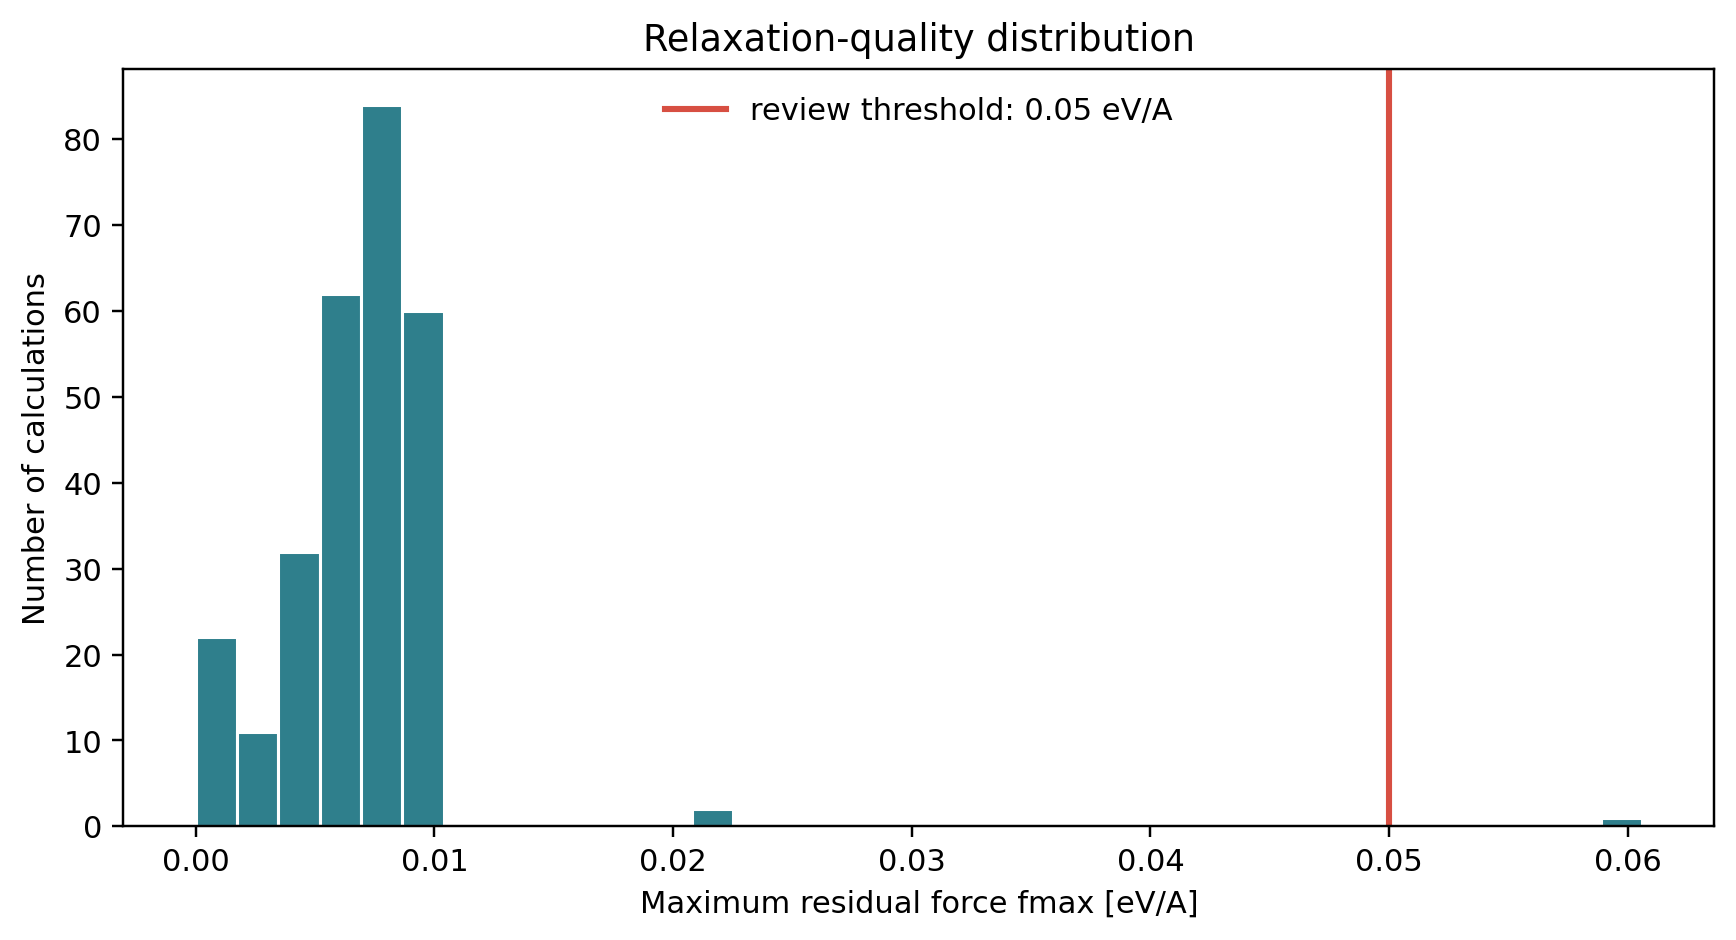
\includegraphics[width=\textwidth]{fmax_distribution.png}
    \end{column}
    \begin{column}{0.42\textwidth}
      \begin{block}{Warum diese Kontrolle wichtig ist}
        Energien sind nur dann sauber vergleichbar, wenn Relaxationen ausreichend konvergiert sind und die zugehoerigen Referenzen stimmen.
      \end{block}

      \begin{itemize}
        \item \texttt{fmax} frueh pruefen
        \item Ausreisser nicht sofort loeschen, sondern erst markieren
        \item Review-Zustand ist didaktisch wertvoll, weil Entscheidungen nachvollziehbar bleiben
      \end{itemize}
    \end{column}
  \end{columns}
\end{frame}

\begin{frame}{Von der Kuration zum wissenschaftlichen Plot}
  \begin{columns}[T,totalwidth=\textwidth]
    \begin{column}{0.58\textwidth}
      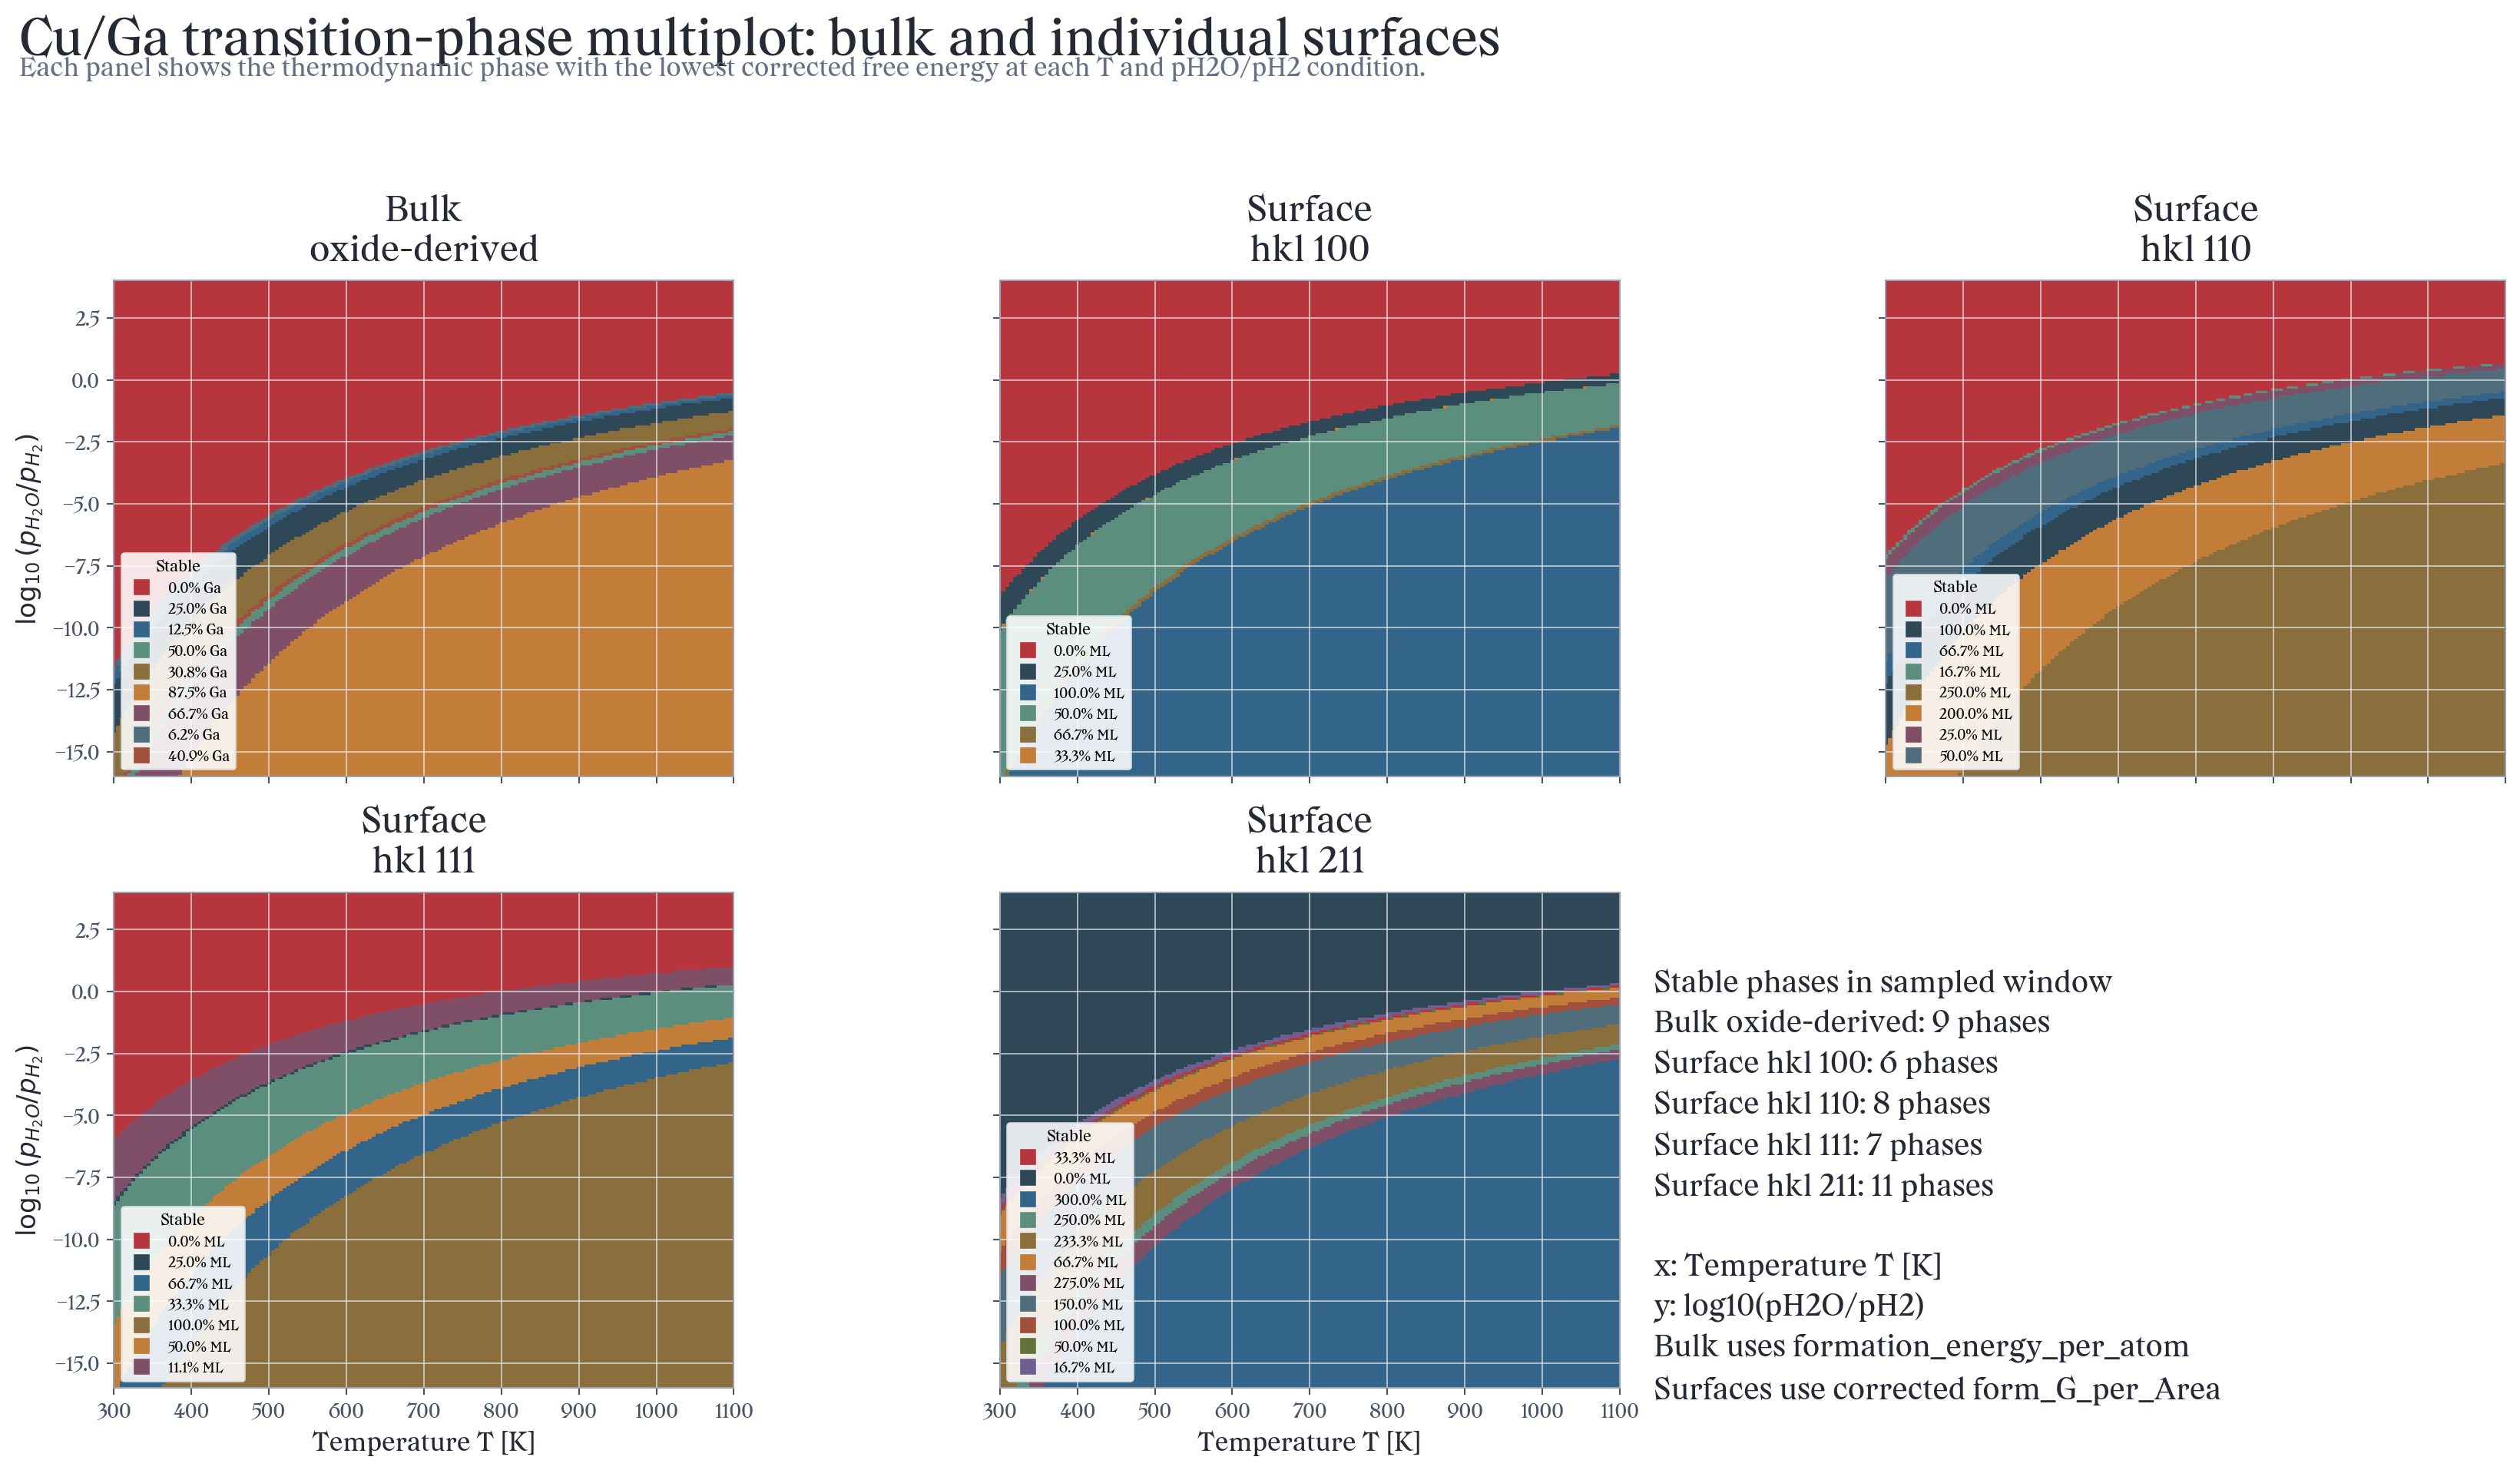
\includegraphics[width=\textwidth]{cuga_bulk_surface_transition_phase_multiplot.png}
    \end{column}
    \begin{column}{0.38\textwidth}
      \begin{itemize}
        \item Visualize zeigt Muster und Ausreisser in den aktiven Daten
        \item Adsorption \& Barriers berechnet chemisch relevante Zielgroessen auf der gefilterten Datenbasis
        \item Jede Interpretation sollte zur auswaehlbaren Einzelrechnung rueckverfolgbar bleiben
      \end{itemize}

      \begin{block}{Didaktische Kernbotschaft}
        Ein Plot ist das Ende eines Weges, nicht der Anfang.
      \end{block}
    \end{column}
  \end{columns}
\end{frame}

\begin{frame}{Empfohlener Arbeitsablauf fuer Studierende}
  \begin{enumerate}
    \item Projekt und Quellen laden
    \item im Workflow nur die noetigen Hilfsspalten bauen
    \item im Controlroom relevante Zeilen eingrenzen
    \item auffaellige Punkte in Records oder ASE einzeln kontrollieren
    \item erst dann Visualize oder Adsorption \& Barriers verwenden
    \item aktive Tabelle und Plot mit kurzer Textnotiz exportieren
  \end{enumerate}

  \vspace{0.4cm}
  \begin{block}{Faustregel}
    Jede Folgerung ueber Stabilitaet, Adsorption oder Barrieren sollte auf eine kleine, kuratierte Untermenge zurueckzufuehren sein.
  \end{block}
\end{frame}

\begin{frame}{Was neue Gruppenmitglieder leicht falsch machen}
  \begin{itemize}
    \item ungefilterte Mischungen aus Testrechnungen, Referenzen und Produktivdaten vergleichen
    \item nur auf die Energie schauen und Struktur oder Referenzzuordnung nicht kontrollieren
    \item leere oder fehlerhafte Formeln als echte chemische Spezies interpretieren
    \item aus Plot-Ausreissern sofort chemische Schluesse ziehen, ohne die Einzelrechnung zu oeffnen
    \item Ausschluesse informell treffen statt ueber den Kurationsstatus zu dokumentieren
  \end{itemize}
\end{frame}

\begin{frame}{Rueckmeldung an den Softwareentwickler}
  \begin{block}{Was bereits stark ist}
    Lokale Datenquellen, strukturierte Filterlogik, ASE-Oeffnung, Adsorptions-Workbench und kuratierbare Row-Actions bilden bereits ein sehr gutes Fundament.
  \end{block}

  \vspace{0.25cm}
  \begin{itemize}
    \item Es fehlt ein klarer Projektassistent fuer Erstnutzer: Daten laden, Namensschema pruefen, Referenzen validieren, erste View speichern
    \item Kuration sollte persistenter und auditierbarer werden: Begruendung, Zeitstempel, Person, Export
    \item Einzelinspektion braucht noch mehr Kontext: direkte Anzeige von Referenzzeile, Nachbarrechnungen und strukturelle Vergleiche
    \item Rechtsklick-artige Aktionen waeren angenehm, wichtiger ist aber eine robuste Kontextleiste fuer ausgewaehlte Zeilen und Plotpunkte
    \item Fuer Lehre waere ein gefuehrter Modus hilfreich: kleine Aufgaben, Warnhinweise und erklaerte Standardabfragen
  \end{itemize}
\end{frame}

\begin{frame}{Fazit}
  \begin{block}{Die wichtigste Lernbotschaft}
    PFUI sollte neuen Studierenden helfen, aus einer lokalen DFT-Datenbank erst eine verstaendliche Arbeitsumgebung und dann eine belastbare wissenschaftliche Aussage zu machen.
  \end{block}

  \vspace{0.4cm}
  \begin{itemize}
    \item gute Nutzung beginnt mit Datenhygiene und Einzelinspektion
    \item ASE und der Controlroom gehoeren in den Alltag, nicht nur in Sonderfaelle
    \item erst kuratierte Daten fuehren zu sinnvollen Energietrends und Phasendiagrammen
  \end{itemize}
\end{frame}

\end{document}
